
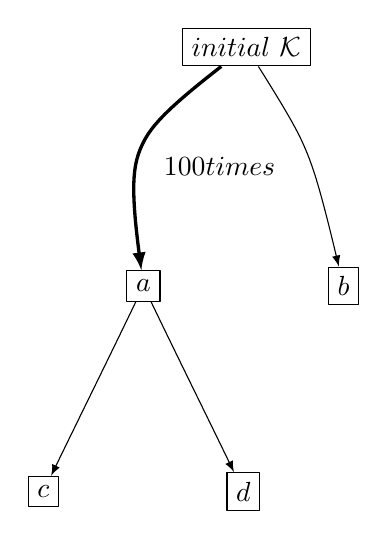
\begin{tikzpicture}[>=latex,line join=bevel,]
%%
\node (a) at (63.0bp,92.0bp) [draw,rectangle] {$a$};
  \node (c) at (27.0bp,18.0bp) [draw,rectangle] {$c$};
  \node (b) at (135.0bp,92.0bp) [draw,rectangle] {$b$};
  \node (root) at (100.0bp,178.0bp) [draw,rectangle] {$initial\  \mathcal{K}$};
  \node (d) at (99.0bp,18.0bp) [draw,rectangle] {$d$};
  \draw [->] (a) ..controls (75.773bp,65.454bp) and (80.995bp,55.009bp)  .. (d);
  \draw [->] (a) ..controls (50.227bp,65.454bp) and (45.005bp,55.009bp)  .. (c);
  \draw [->] (root) ..controls (114.96bp,154.18bp) and (118.41bp,147.98bp)  .. (121.0bp,142.0bp) .. controls (124.02bp,135.05bp) and (126.58bp,127.27bp)  .. (b);
  \draw [->,very thick] (root) ..controls (70.045bp,154.73bp) and (65.108bp,148.72bp)  .. (62.169bp,142.0bp) .. controls (59.204bp,135.22bp) and (58.35bp,127.39bp)  .. (a);
  \definecolor{strokecol}{rgb}{0.0,0.0,0.0};
  \pgfsetstrokecolor{strokecol}
  \draw (90.416bp,135.0bp) node {$100 times$};
%
\end{tikzpicture}
